\begin{frame}
  \frametitle{Results for the Previous Week}

  \begin{center}
    Here are the results for last week:

    \bigskip
    
    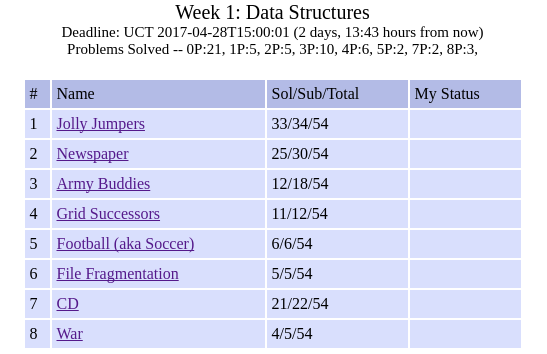
\includegraphics[width=0.8\textwidth]{img/resultsW1}

    \bigskip

    Please make sure that your results appear correctly in My
    Status. If they don't, maybe I don't have your UVA ID!
  \end{center}
\end{frame}

\begin{frame}[fragile]
  \frametitle{Pre-class Notes 1/3 -- Java}

  \begin{block}{Java Speed}
    Some students had problems with JAVA getting TLE (time limited
    exceeded).

    \bigskip

    Java I/O functions {\bf can be slow}. Use the following tricks to
    speed things up:
  \end{block}

  \begin{itemize}
  \item Don't use \emph{System.out.println} -- Use
    \emph{BufferedWriter} instead: 90\%
    speedup!\footnote{\url{https://www.redgreencode.com/why-is-java-io-slow/}}
  \item Don't use \emph{Scanner} -- Use \emph{BufferedReader} instead: 80\% speedup!
  \end{itemize}
\end{frame}

\begin{frame}[fragile]
  \frametitle{Pre-class Notes 1/3}

  \begin{block}{Java Speed}
    Some students had problems with JAVA getting TLE (time limited
    exceeded).

    \bigskip

    Java I/O functions {\bf can be slow}. Use the following tricks to
    speed things up:
  \end{block}

  \begin{itemize}
      \item Don't add strings in a loop:
    {\small
\begin{verbatim}
String a,b;
for (int i = 0; i < N; i++) { a = a + b; } // SLOW!
\end{verbatim}
    }
  \item Use \emph{StringBuilder} instead:
    {\small
\begin{verbatim}
StringBuilder sb; String a,b;
for (int i = 0; i < N; i++) { sb.append(b); }
a = sb.toString();
\end{verbatim}
    }
  \end{itemize}
\end{frame}

\begin{frame}[fragile]
  \frametitle{Pre-class Notes 1/3}

  \begin{block}{Java Speed}
    Some students had problems with JAVA getting TLE (time limited
    exceeded).

    \bigskip

    Java I/O functions {\bf can be slow}. Use the following tricks to
    speed things up:
  \end{block}

  \begin{itemize}
      \item Java \emph{Arraylist}'s {\bf contain()} is O(n)\footnote{\url{http://stackoverflow.com/questions/10196343/hash-set-and-array-list-performances}}
    {\small
\begin{verbatim}
ArrayList<Int> a;
for (int i = 0; i < N; i++) { a.contain(b); }
\end{verbatim}
    }
  \item Use \emph{HashMap} instead (O(1)):
    {\small
\begin{verbatim}
HashMap<Int> a;
for (int i = 0; i < N; i++) { a.contain(b); }
\end{verbatim}
    }
  \end{itemize}
\end{frame}

\begin{frame}
  \frametitle{Pre-class Notes 2/3 -- Python}
  \begin{block}{Python Speed}
    Some students are also having problems with PYTHON getting
    TLE. (Problems CD and Newspaper).
  \end{block}

  \begin{itemize}
  \item Unfortunately, I could not find any good hints in Python.

  \item Did anyone manage to get {\bf Accepted} in python for these
    two problems?
  \end{itemize}
\end{frame}

\begin{frame}
  \frametitle{Pre-class Notes 3/3 -- Golden Week}

  \begin{itemize}
  \item No class 5/1 -- Monday Class is {\bf 5/8}
    \vfill
  \item Deadline for Week 2 is {\bf 5/12}
    \vfill
  \item Have a fun Golden Week!
  \end{itemize}
\end{frame}



% Java Speed
% Python Speed
% Java ASCII characters
% Golden Week
